% Mission elements section
% File: sections/mission_elements.tex
\documentclass[../main.tex]{subfiles}

\begin{document}

\section{Mission elements}\label{mission-elements}
TBD

\subsection{Mission description}\label{mission-description}

TBD

\subsection{Requirements}\label{requirements}

TBD

% Requirements table and instructions

\emph{Create at least 9 different requirements from a `ECSS Requirement
categories'' perspective, and 8 different requirements from a `Product
Breakdown Structure (PBS)' perspective. Note that this can be combined,
so you could only have 9 requirements in total if you find the right
combinations. Also include the type (key, killer, driving, normal), the
rationale, the verification method (Inspection, Demonstration, Test,
Analysis, By similarity, Simulation and modeling (Design)) and if
applicable, an ECSS document reference.}

\textbf{Reference documents}
\begin{table}[htp]
\centering
% \renewcommand{\arraystretch}{1.2} % row height
\begin{tabularx}{\textwidth}{|p{0.6cm}|X|p{1.5cm}|p{2cm}|p{1cm}|p{2cm}|p{1.2cm}|p{1.4cm}|}
\hline
Req. ID & Description & Rationale & ECSS Req. Category & Type & Applicable PBS level/item & V\&V method & ECSS doc. reference \\
\hline
& & & & & & & \\
\hline
& & & & & & & \\
\hline
& & & & & & & \\
\hline
& & & & & & & \\
\hline
& & & & & & & \\
\hline
& & & & & & & \\
\hline
& & & & & & & \\
\hline
\end{tabularx}
\end{table}

\subsection{Concept designs}\label{concept-designs}

TBD

\subsection{System and subsystem level trade-offs leading to final
concept
design}\label{trade-offs}

TBD

\subsection{Description of system
elements}\label{description-of-system-elements}

TBD

\subsection{Product Breakdown Structure
(PBS)}\label{pbs}

TBD

\emph{Below is an example of an 8 levels PBS with generic names in the
boxes. Replace the names with items from your chose concept design, and
preferably also the system and subsystem that you do a trade-off for.
Give the items a unique number that you can also insert in the
requirements table.}

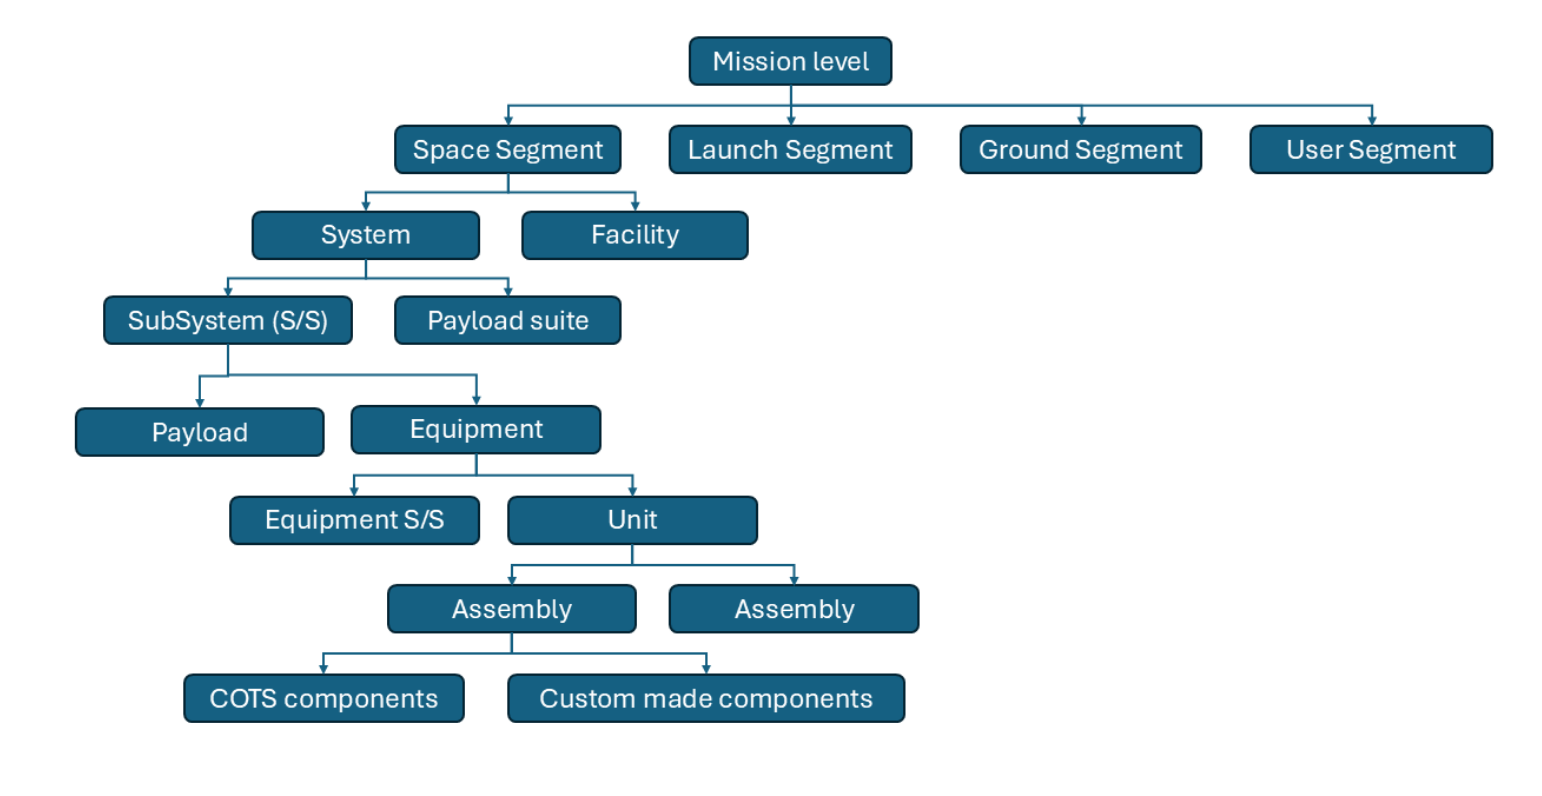
\includegraphics[width=6.28264in,height=3.53403in]{media/Product Breakdown Structure.png}

\subsection{Verification and Validation of
requirements}\label{verification-and-validation}

TBD

\end{document}
